\documentclass{MScthesisITEM}

% this package is just to generate text for demo-purposes

\usepackage{blindtext}
\usepackage{mathtools} % math packages
\usepackage[siunitx]{circuitikz}
\usepackage{todonotes}
\usepackage{hyperref}
\usepackage{subcaption}
\usepackage{listings}
\usepackage{wrapfig}
\usepackage{pgfplots}
\usepackage{filecontents}
\usepackage{url}

%\pgfplotsset{compat=1.11}

\lstset{
	numbers=left,
	stepnumber=1, 
	numbersep=5pt,
	showspaces=false,
	showstringspaces=false,
	showtabs=false,
	basicstyle=\footnotesize, 
	numberstyle=\footnotesize, 
	tabsize=2, 
	breaklines=true,
	captionpos=b,}

\title{Named Data Networking} % The title of your assignement; NB use \newlinetitle to start a newline
\author{Haakon Garseg Mørk} % Your firstname and lastname
\professor{Stig F. Mjølsnes, ITEM} % Affiliation = ITEM for instance
\supervisor{N/A}

%% Uncomment the following in case you want subfigures; note that there will be a warning for the caption package
% \let\subcaption\undefined
% \let\subfloat\undefined
% \usepackage[bf]{caption}
% \usepackage{subcaption}

\DeclareGraphicsExtensions{.pdf,.jpg}
\graphicspath{{./figs/}}

\loadglsentries{glossary}
\makeglossaries

\begin{document}
\selectlanguage{english}
\pagenumbering{roman}
\pagestyle{plain}

%% Only for the project; comment out the line below for the master's thesis; the front page will be generated automatically by DAIM
\titleITEM

%% Only for the master's thesis; for the project report the description is taken from It's Learning and added by the department
% \selectlanguage{english} % Change to 'norsk' if you are writing in Norwegian
% \begin{titlingpage}

\noindent
\begin{tabular}{@{}p{4cm}l}
\textbf{Title:} 	& Identity-Based Trust Model in Named Data Networking \\
\textbf{Student:}	& Haakon Garseg Mørk \\
\end{tabular}

\vspace{4ex}
\noindent\textbf{Problem description:}
\vspace{2ex}

The translation from name to address and location is a fundamental problem to all networks.
Named Data Networking (NDN) is a proposal for content-centric discovery and routing approach to networking
going on at the University of California, Los Angeles (UCLA) [1], which is part of the inspiration and a contact point for this work.

This project aims to understand the ideas and concepts of named data networking, and investigate the
potential these notions hold for network security, even for properties of anonymity and privacy. 
The student work should be to build a public key distribution application that uses ChronoSync [2] and runs over NDN.
This approach will allow for easy experimentation in the regular internet protocols environment.     

[1]  UCLA.  Named Data Networking. Web site at http://named-data.net/

[2]  UCLA, Named-data Networking. ChronoSync https://github.com/named-data/ChronoSync

\noindent
\begin{tabular}{@{}p{4cm}l}
\textbf{Responsible professor:} 	& Stig F. Mjølsnes \\
\textbf{Supervisor:}			& Stig F. Mjølsnes \\
\end{tabular}

\end{titlingpage}
% \cleardoublepage

%% There must be an abstract in English, even though the main text is in Norwegian
\selectlanguage{english}
\pagestyle{empty}
\begin{abstract}
Abstract goes here...
\end{abstract}
\cleardoublepage

%% Only for the master's thesis; if the main text is in English and you can write Norwegian, there must be an abstract in Norwegian as well.
% \selectlanguage{norsk}
% \pagestyle{empty}
\begin{abstract}

IP nettverket ble bygd for flere ti\r{a}r siden, og med dagens bruk av Internet ser vi at en ny nettverksprotokoll er s\r{a}rt trengt.
Named Data Networking (NDN) er en foresl\r{a}tt nettverksprotokoll som baserer seg p\r{a} innhold, istedenfor punkt-til-punkt arkitekturen som er grunnlaget for IP.
Selv med flere ti\r{a}rs bruk av Internet, er enn\r{a} ikke problemene med Public Key Infrastructure (PKI) l\o{}st. 
I NDN, har man heller ikke klart \r{a} finne en l\o{}sning p\r{a} dette.
Identitetsbasert kryptografi (IBC) viser seg \r{a} være anvendelig til tr\r{a}dl\o{}se sensornettverk, og enda mer n\r{a}r sensornettverket kj\o{}rer over NDN.

I denne masteroppgaven forklarer jeg NDN arkitekturen og de grunnlegende prinsippene i IBC.
Jeg modellerer og implementerer en applikasjon for \r{a} demonstrere bruken av IBC over NDN i et tenkt sensornettverk.

Implementasjonen og testingen av mitt bidrag verifiserer relevansen av IBC i et sensornettverk som kj\o{}rer over NDN, samt brukervennligheten rundt det \r{a} utvikle applikasjoner over NDN.

Jeg formelt og uformelt beviser sikkerheten i protokollene som er foresl\r{a}tt til enhetsregistrering og data foresp\o{}rsel i applikasjonen.

\end{abstract}
% \cleardoublepage

\selectlanguage{english}% Change to 'norsk' if you are writing in Norwegian

% \renewcommand{\abstractname}{Preface}
\begin{abstract}
\noindent \blindtext 
\end{abstract}
% \cleardoublepage

\renewcommand{\abstractname}{Acknowledgments}
\begin{abstract}
I am eternally grateful for the support of my fellow student, Eirik Auran Rathe.
Mr. Rathe has helped me with extraordinary suggestions, different approaches, and last but not least, his dick in my ass.

\end{abstract}
\cleardoublepage

% similarly you may add a separate acknowledgments page

\tableofcontents*
\cleardoublepage

%% include if relevant
\listoffigures
\cleardoublepage

\lstlistoflistings
\cleardoublepage

%% include if relevant
\listoftables
\cleardoublepage

%% include if relevant
% \listofalgorithms
% \addcontentsline{toc}{chapter}{List of Algorithms}
% \cleardoublepage

%% include if relevant
% \printglossary[title=List of Symbols, style=long]
% \cleardoublepage
% \glsaddall[]

% include if relevant
\printglossary[title=List of Acronyms,type=\acronymtype] % prints just the list of acronyms
\cleardoublepage

\pagenumbering{arabic}
\pagestyle{ruled}
\chapter{Introduction}\label{chp:introduction} 

\section{Motivation}
The translation from name to address and location is a fundamental problem to all networks.
\gls{NDN} is a proposal for content-centric discovery and routing approach to networking
going on at the \gls{UCLA}, which is part of the inspiration and a contact point for this work.

In general, the name to address resolution can either be maintained by a catalogue lookup service, 
such as \gls{DNS} (Internet) and \gls{HLR} (mobile networks), 
or resolved on-the-fly by a protocol on request, such as \gls{ARP} (\gls{LAN}). 
There has been a tremendous amount of work done on the naming problem in distributed systems, 
some became big failures (e.g. X.500) others such as the web \gls{URL}s are very successful. 
Bringing things even further, the \gls{DOI} system is a \gls{URI} directed at the content/object itself rather than a location. 
Very much related to the name/address problem is the information security problem of efficient and practical public key distribution, 
which remain unsolved in practice, even though a significant number of digital certificate and verification protocols and schemes have been proposed, and systems tested over the last two decades. 
One notable and early theoretical proposal is Rivest and Lampson \gls{SDSI} proposal~\cite{rivest1996sdsi},
and subsequent work, that may be revisited for applicable to named data networking.

\section{Problem and Scope}

When designing a new network protocol for the future Internet, one of the most significant changes should be that it is designed for security.
Trust management plays a big part in security, and thus we cannot design trust management on known \gls{IP} failures such as X.500. 
\gls{PKI} is a tough challenge to solve and the solution is probably not the one or the other, but rather case specific.

I address the trust management issue in a though sensor device network, e.g. a health sensor network.
By using the \gls{NFD} I will implement my proposal for such a sensor network.

\section{Methodology}

First I find in what context the Public Key System can be applicable, then I design the application flow in sequence diagrams.
Based on how \gls{NDN} is designed, I try to implement the proposed design and see where to redesign the application proposal for achieving minimal communication overhead, security (i.e. \gls{CIA}) and usability.

\section{Outline}

This paper will first introduce one of the proposed protocols for the future Internet, \gls{NDN}.
I will explain the architecture of \gls{NDN} as well as some related work regarding my application proposal. 
The application modules will be explain in detail and implementation choices will be discussed.
At last I will present the results of the implementation and my conclusion of the trust model.
\chapter{Background}\label{chp:background} 
Ingress


\section{Information-Centric networking}\label{chp2:sec:icn}
\gls{ICN} ...


\section{NDN Architecture}\label{chp2:sec:ndn_architecture}
\gls{NDN} ...

\subsection{Naming}
Naming is left to the application design.
\chapter{Experimental Setup}\label{chp:experimental_setup}
Ingress


\section{ChronoSync}
ChronoSync~\cite{DBLP:conf/icnp/ZhuA13}
Encode data into crypto digest, i.e. a state digest, to exchange states between all parties. 
If the state is equal to the one stored locally, then nothing should happen.
If not, two options are available; 
- the differences of the dataset state can be directly inferred
and sent as the response to the sync interest if the state
digest is the same as one of the previous local state
digests;
- a state reconciliation method is used to determine the dif-
ferences of the knowledge if the state digest is unknown
(for example, when recovering from a network partition).

Sync interest
Sync data
Recovery interest
Recovery data

\section{Identity-based cryptography}
Identity-based cryptography~\cite{DBLP:conf/icnp/ZhangCXWSW11}
\chapter{..}

\section{Public Key Distribution}
Instead of the PKI, where each pk is signed by a certificate authority and the generated certificate is sent as a response in https, then validated by the the client, we want to make the certificate authority obsolete by distributing every PK and rather trust the name (e.g. /ntnu/). 

\subsection{Key Revocation}
Key Revocation becomes obsolete with Public Key Sync. 

\section{Information Based Cryptography}
\gls{IBE} presented by Shamir~\cite{DBLP:conf/crypto/Shamir84} in 1984.

Thoroughness of the name allocation \gls{NRS} 
Identity-based cryptography~\cite{DBLP:conf/icnp/ZhangCXWSW11} in \gls{NDN}

Key Revocation in IBE ~\cite{DBLP:journals/iacr/BoldyrevaGK12}

Drawbacks
If \gls{PKG} is compromised. Adversary has private key to all nodes that used the compromised \gls{PKG}
\gls{PKG} can read and write messages related to the node, because it has all private keys, i.e. \gls{MITM}.
\gls{PKG} and the requesting node has to establish a secure channel. 

\subsection{..}
Name sync (same application as Public Key Sync).

\chapter{Results}\label{chp5:results}

\chapter{Discussion}
In this chapter the work done in conjunction to this thesis will be discussed. 
First I will talk about the pros and cons using \gls{IBC} in \gls{NDN}.
Then I will discuss the \gls{HSS} and possible drawbacks in the system. 
Scalability issues and other applicable networks for the application will be mentioned.

\section{Identity-Based Cryptography in Named Data Networking}
Concerning key revocation, one suggestion has been to add a monthly timestamp to the \gls{name}, but the the \gls{PKG} has to renew private keys for everybody each month. 
This solution do not scale very well due to a lot of computation at the \gls{PKG}.
With the \gls{FSM}, every user will be notified when a identity is revoked.
There is no use for periodically checking names.
But the renewal of keys might not be an issue in the \gls{HSS}. \todo{more..}

\todo{refactor this section}
Can authenticate \gls{data} even using insecure DNS or HTTP. 
There is only one linkage between the \gls{name} and the content, and if the user obtains the right \gls{MPK}, there is no doubt where the \gls{data} originates from and that it is not altered.
In RSA public key cryptography we have to find the key related to the signature. 
In worst case this will be equivalent of retrieving the \gls{MPK} each time, which is not likely. 
Or the \gls{MPK} can be appended to the message.

usability 



\section{Development Usability in Named Data Networking}
Once a basic perception of the \gls{NDN} architecture is understood, it is easy to begin developing.
The \gls{PyNDN2} framework comes with good examples of how to develop simple applications with packets that are signed and encrypted.

The concept of naming \gls{data} introduces more simplicity, but also a new way of application design thinking.
Addressing is dealt with one place in the architecture compared to an equivalent system over \gls{IP}. 
Security is easily applied in \gls{NDN}.

\section{Health Sensor System}
The application is not tested on with real sensors, hence I cannot conclude with anything regarding the computational power of such devices, nor the life time of the battery when performing \gls{IBE}.  

Power efficiency
\todo{more on this}

A problem with \gls{wsn} in \gls{IP} networks, is that it is a limited number of \gls{IP} adderesses (especially in \gls{IPv4}).
So the global scalability issue arises due to the potentially large number of sensors that could be deployed. 
With the naming rules in \gls{NDN}, this is not a issue.

In~\autoref{ibc-performance} we can see that \gls{IBC} is performing better than regular asymmetric cryptography, RSA. 

Encrypting with same symmetric key for each set of \gls{data}, limits the encryption computation for the device if several devices requests the same \gls{data}.
Using a unique key for each time \gls{data} is requested is more secure and can be used for more sensitive content.

Who can play the role of a device?
As mentioned in~\autoref{rendezvous_authentication} and~\autoref{init} there should be a limitation of which devices that can be initialized to the trust domain.
\todo{hm... something here?}

Storing the \gls{SK} in a secure fashion.

Preloading secret key, offline mode, yet the initialization protocol should be used to do this, unless the sharing is done in a wired environment. 
\gls{NFC} signal is hard (impossible?) to eavesdrop, thus the initialization protocol is not needed. 


\section{Scalability}
Distributing the \gls{ID}-list can be an issue, as the list can grow linearly with the number of participants in the trust domain.
However, this might not be a huge problem in the use cases that is addressed in this thesis, considering that the number of devices in the \gls{HSS} will not grow larger than e.g. 100 devices. 

\section{Sync}
The sync application makes it possible for users to know who has a valid public key within the \gls{PKG}s domain.
One drawback with the key distribution using \gls{FSM} is that for the sender to be 100\% sure that the message is encrypted with the latest \gls{ID}, the sender has to rely on that it has received the latest sync state available from the \gls{PKG}.
Likewise when a \gls{receiver} verifies a signature, it has to rely on the same principle to be able to know if the belonging \gls{ID} is still valid.
Since the scalability is not that big of an issue in this scenario, the monthly (or even more often) timestamp appended to the \gls{ID} might be a good solution to reduce the time of exposure when compromised.

There are some issues that could occur in such a system. 
\gls{DoS} on Sync \gls{interest} and Sync \gls{data}. 
If the \gls{FSM} is used to revoke public keys as suggested, an attacker who has found the compromised \gls{SK}, can try to deny the distribution of the new list, i.e. the Sync \gls{data}, from the distributor. 
This is however a complicated attack and an updated list would spread fast.
Performing \gls{DoS} on every node is not easy, and would block the network access for the adversary anyway.
In~\cite{DBLP:conf/spw/StajanoA99} Frank Stajano and Ross Anderson mentions possible \gls{DoS} attacks, such as radio jamming and battery exhaustion. 
All applications that relies on some sort of crucial information derived using \gls{FSM} (\autoref{file-sync}) are vulnerable to this kind of \gls{DoS}.

\section{Other Use Cases}
The trust model used in the \gls{HSS} can be used in any network where the use of a \gls{TTP} is accepted. 
Such a system can for instance be:
\begin{enumerate}
	\item Home automation systems
	\item \gls{BAS}
	\item \gls{BMS}
	\item Health care
	\item Military networks
	\item Sensor networks such as disaster, habitat and hazard monitoring
\end{enumerate}



\chapter{Conclusion and Future Work}\label{chp7:conclusion}
\chapter{NDN node 23 - NTNU}

\section{NDN node 23 - NTNU}
Node 23 in NDN testbed

\begin{figure}[ht]
  \centering
  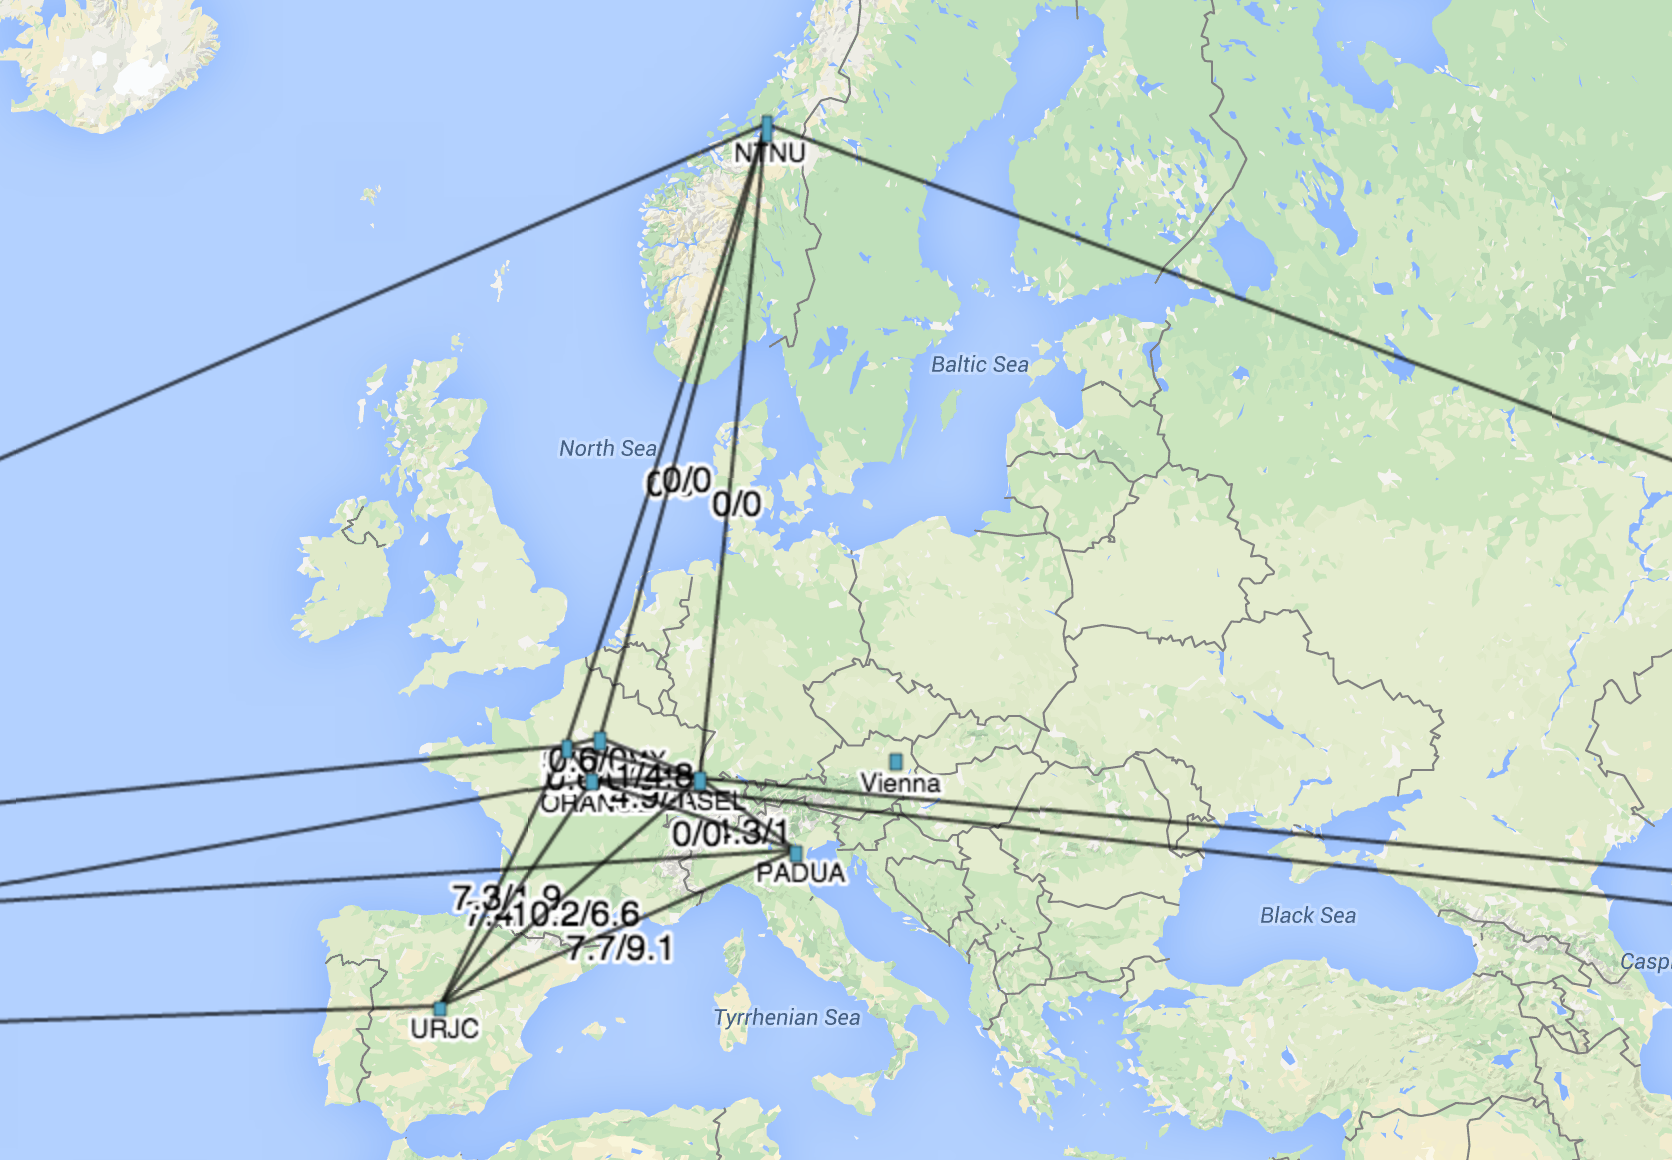
\includegraphics[width=1\textwidth]{ndn-map.png}
  \caption{NDN Map}
  \label{fig:ndn-map}
\end{figure}

%% include here the other chapters

%% References
%\include{references}
\renewcommand*{\bibname}{References}
%\bibliographystyle{ieeetr}
\bibliographystyle{alpha}
\bibliography{main}

% Uncomment the following if you have any appendix
\appendix
\addtocontents{toc}{%
 \protect\vspace{1em}%
 \protect\noindent \bfseries \appendixtocname\protect\par
 \protect\vspace{-.5em}%
}
\renewcommand{\chaptername}{\appendixname}
% include below possible appendices (chapters)
%\include{appendix}
\chapter{Code}\label{apx:code}

\lstset{language=Python, 
    basicstyle=\ttfamily\small, 
    keywordstyle=\color{keywords},
    commentstyle=\color{comments},
    stringstyle=\color{red},
    showstringspaces=false,
    %procnamekeys={def,class}
    identifierstyle=\color{green}
    }

\section{Scyther Security Analysis of Device Registration}\label{apx:scyther-analysis-dr}
To better understand the code,~\autoref{tbl:mapping_code} is presents mapping of the~\autoref{fig:init_ibe_2} to the code.

\begin{table}[h]
  \begin{tabular}{lll}
  Figure      				& SPDL Code     			& Description 				\\ \hline
  ID\textsubscript{d}  		& D   						& Identity of the device 	\\ %\hline
  ID\textsubscript{PKG}   	& PKG      					& Identity of the PKG 		\\ %\hline
  n      					& R            				& Random nonce 				\\ %\hline
  sk      					& SK           				& Secret key to an identity	\\ %\hline
  c\textsubscript{1} = AES\_Enc\textsubscript{tk}[ID\textsubscript{d} || n]  & c1 = \{ D, R \}k(PKG,D)   & AES encrypted content		\\ %\hline
  c\textsubscript{2} = AES\_Enc\textsubscript{tk}[sk || \~{n}]     	& c2 = \{ SK, R \}k(PKG,D)	& AES encrypted content 	\\ %\hline
  s = Sign(mpk || sk\textsubscript{pkg} || c\textsubscript{2})      & s = \{ SHA1(c2) \}sk(PKG)   & Signature				\\ %\hline
  \end{tabular}
  \caption{Mapping of the~\autoref{fig:init_ibe_2} and the \gls{spdl} code.}
  \label{tbl:mapping_code}
\end{table}

\begin{lstinputlisting}
[language=Python]{../src/device_registration.spdl}
\end{lstinputlisting}

\clearpage
\section{Scyther Security Analysis of Data Pull}\label{apx:scyther-analysis-dp}
To better understand the code,~\autoref{tbl:mapping_code_data} is presents mapping of the~\autoref{fig:data_pull_ibe} to the code.

\begin{table}[h]
  \begin{tabular}{lll}
  Figure      				& SPDL Code     			& Description 				\\ \hline
  ID\textsubscript{d}  		& D   						& Identity of the device 	\\ %\hline
  ID\textsubscript{m}   	& M      					& Identity of the mobile	\\ %\hline
  n      					& R            				& Random nonce 				\\ %\hline
  sk      					& SK           				& Secret key to an identity	\\ %\hline
  c\_cek = Encrypt(mpk || ID\textsubscript{d} || cek)	& ccek = \{ cek \}pk(D) 		& IBEncrypted CEK 	\\
  c = AES\_Enc\textsubscript{cek}(data || \~{n}) 		& c = \{ data , R \}k(M,D) 	& AES encrypted content 	\\
  m\textsubscript{1} = (ID\textsubscript{d} || n || request)  & m1 = (M, D, R)   	& Message		\\ %\hline
  c\textsubscript{2} = (c\_cek || c)     	& c2 = (M, c, ccek)						& Message 	\\ %\hline
  s\textsubscript{1} = Sign(mpk || sk\textsubscript{m} || c\textsubscript{1})      	& s1 = { SHA1(m1) }sk(M)   & Signature				\\ %\hline
  s\textsubscript{2} = Sign(mpk || sk\textsubscript{d} || c\textsubscript{2}      	& s2 = { SHA1(c2) }sk(D)   & Signature				\\ %\hline
  \end{tabular}
  \caption{Mapping of the~\autoref{fig:init_ibe_2} and the \gls{spdl} code.}
  \label{tbl:mapping_code_data}
\end{table}

\begin{lstinputlisting}
[language=Python]{../src/data_pull.spdl}
\end{lstinputlisting}

% \section{File Sync}\label{apx:file-sync-code}

% Using watchdog to observe files

% \begin{lstinputlisting}
% [language=Python]{../../master-thesis-work/fileSync.py}
% \end{lstinputlisting}

% \section{Device}\label{apx:device-code}

% Device, e.g. a sensro device or a mobile.

% \begin{lstinputlisting}
% [language=Python]{../../master-thesis-work/device.py}
% \end{lstinputlisting}

% \section{Public Key Generator}\label{apx:pkg-code}

% \gls{PKG}

% \begin{lstinputlisting}
% [language=Python]{../../master-thesis-work/publicKeyGenerator.py}
% \end{lstinputlisting}

% \section{Identity-Based Encryption}\label{apx:ibe-code}

% \gls{IBE}

% \begin{lstinputlisting}
% [language=Python]{../../master-thesis-work/identityBasedCrypto.py}
% \end{lstinputlisting}

% \section{Main}\label{apx:main-code}

% Main..

% \begin{lstinputlisting}
% [language=Python]{../../master-thesis-work/application.py}
% \end{lstinputlisting}

% \section{Message Buffer Protocol}\label{apx:msgBuf-code}
% \begin{lstinputlisting}
% [language=XML]{../../master-thesis-work/messageBuf.proto}
% \end{lstinputlisting}

\end{document} 
